\section{Hurwitz}
The genus formula of \href{http://en.wikipedia.org/wiki/Bernhard_Riemann}{Bernhard Riemann} (on the left in Figure~\ref{figure:riemann-hurwitz}) and \href{http://en.wikipedia.org/wiki/Adolf_Hurwitz}{Adolf Hurwitz} (on the right in Figure~\ref{figure:riemann-hurwitz}) asserts that if~$\phi\colon C_1 \rightarrow C_2$ is a separable cover of curves, we have an inequality relating their genera:
\begin{equation}
  \label{equation:riemann-hurwitz}
  2 \genus_{C_1} - 2 \geq \deg(\phi)(2 \genus_{C_2} -2) + \sum_{P \in C_1} (e_{\phi}(P)-1)
\end{equation}

\begin{figure}[hb]
  \centering
  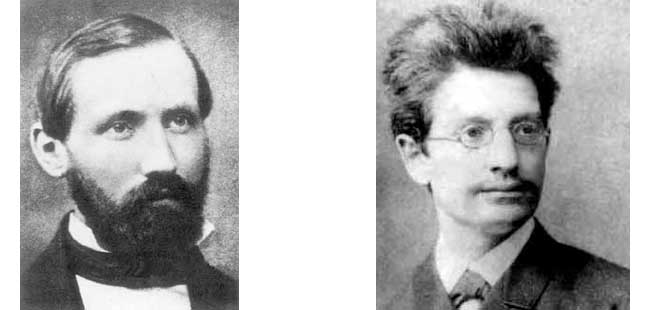
\includegraphics[width=10cm]{0-geometry/riemannhurwitz}
  \caption{Bernhard Riemann and Adolf Hurwitz}
  \label{figure:riemann-hurwitz}
\end{figure}

Let's first understand all these terms. The cover~$\phi\colon C_1 \rightarrow C_2$ is separable if the induced field-extension~$\phi^{\ast}(\overline{k}(C_2)) \subset \overline{k}(C_1)$ is finite and separable. The dimension~$[\overline{k}(C_1) : \phi^{\ast}(\overline{k}(C_2))]$ is called the degree of~$\phi$. By using a discriminant argument as in Section~\ref{section:genus} we know that for all but finitely many points~$Q \in C_2$ there are exactly~$\deg(\phi)$ points of~$C_1$ lying over it.

In general, let~$P \in C_1$ with corresponding discrete valuation ring~$\mathcal{O}_P$ in~$\overline{k}(C_1)$, then~$\mathcal{O}_P \cap \phi^*(\overline{k}(C_2))$ is a discrete valuation ring in~$\overline{k}(C_2) \simeq \phi^*(\overline{k}(C_2))$ and thus of the form~$\mathcal{O}_Q$ for some~$Q \in C_2$. Naturally we have~$\phi(P)=Q$.

If~$R$ is the integral closure of~$\mathcal{O}_Q$ in~$\overline{k}(C_1)$, then~$R$ is a semi-local Dedekind domain and a PID. If~$t_Q$ is a uniformizer of~$\mathcal{O}_Q$ we have
\begin{equation}
  (t_Q) = P_1^{e_1} \cdots P_r^{e_r}
\end{equation}
where the~$P_i$ are the maximal ideals of~$R$ which corresponds to points~$P_i \in C_1$. The integer~$e_i$ is called the ramification index of~$\phi$ in~$P_i$ and will be denoted~$e_{\phi}(P_i)$. Clearly we have that~$\deg(\phi) = \sum_i e_{\phi}(P_i)$. 

\begin{figure}[ht]
  \centering
  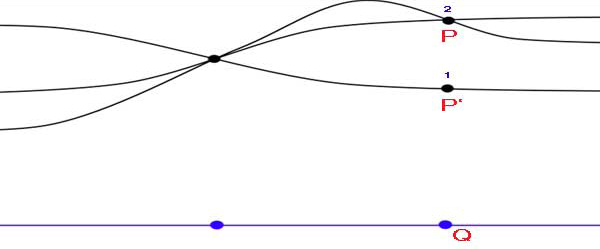
\includegraphics[width=10cm]{0-geometry/ramification}
  \caption{Ramification visualized}
  \label{figure:ramification-visualized}
\end{figure}

Further, for almost all~$P \in C_1$ we will have~$e_{\phi}(P)=1$. With these notations we can now begin the

\begin{proof}[Proof of the Riemann-Hurwitz inequality]
Because~$\phi$ is separable, we have an inclusion
\begin{equation}
  \phi^*\colon\Omega_{C_2} \hookrightarrow \Omega_{C_1} \qquad \phi^*(f\,\mathrm{d}x)=\phi^*(f)\,\mathrm{d} \phi^*(x)
\end{equation}

Take a point~$Q \in C_2$ with uniformizer~$t_Q \in \mathcal{O}_Q$ and write~$\omega = f\,\mathrm{d}t_Q \in \Omega_{C_2}$. For the finitely many~$P_i \in C_1$ lying over~$Q$ we have (as before) that~$\phi^*(t_Q) = u t_{P_i}^{e_i}$ with~$e_i = e_{\phi}(P_i)$ and~$u$ a unit in the discrete valuation ring~$\mathcal{O}_{P_i}$. But then,
\begin{equation}
  \begin{aligned}
    \phi^*(\omega) &= \phi^*(f)\,\mathrm{d} \phi^*(t_Q) \\
    &= \phi^*(f)\,\mathrm{d}(u t_{P_i}^{e_i}) \\
    &= \phi^*(f)\left(e_i u t_{P_i}^{e_i-1} + \frac{\mathrm{d}u}{\mathrm{d}t_{P_i}} t_{P_i}^{e_i}\right)\,\mathrm{d}t_{P_i}.
  \end{aligned}
\end{equation}

The valuation~$\operatorname{ord}_{P_i}$ of~$e_i u t_{P_i}^{e_i-1}$ is~$e_i-1$ (unless~$e_i=0$  in~$k$, that is~$\character(k) \divides e_i$) whereas the valuation of~$(\tfrac{\mathrm{d}u}{\mathrm{d}t_{P_i}}) t_{P_i}^{e_i}$ is~$\geq e_i$. But then,
\begin{equation}
  \begin{aligned}
    \operatorname{ord}_{P_i}(\phi^* \omega) &\geq \operatorname{ord}_{P_i}(\phi^*(f)) + e_i -1 \\
    &= \operatorname{ord}_Q(f) e_i + e_i - 1 \\
    &= \operatorname{ord}_Q(\omega) e_{\phi}(P_i) + e_{\phi}(P_i) -1
  \end{aligned}
\end{equation}

Summing these inequalities over all~$P \in C_1$ we get for the degree of the divisor
\begin{align}
  \deg\left( \operatorname{div}(\phi^*(\omega)) \right) &\geq \sum_{P \in C_1} \left(e_{\phi}(P) \operatorname{ord}_{\phi(P)}(\omega)+e_{\phi}(P) -1 \right) \\
  &=\sum_{Q \in C_2} \left( \sum_{P \in \phi^{-1}(Q)} (e_{\phi}(P) \operatorname{ord}_Q(\omega) + e_{\phi}(P) -1) \right) \\
  \intertext{and because we already know that~$\deg(\phi) = \sum_{P \in \phi^{-1}(Q)} e_{\phi}(P)$ for all~$Q \in C_2$, this is equal to}
  &=\left( \sum_{Q \in C_2} \deg(\phi) \operatorname{ord}_Q(\omega) \right)+\left( \sum_{P \in C_1} (e_{\phi}(P)-1) \right) \\
  &=\deg(\phi)\deg(\operatorname{div}(\omega)) + \sum_{P \in C_1} (e_{\phi}(P)-1).
\end{align}

Plugging in the relation between the genus and the degree of the divisor of a nonzero differential form, we have here the Riemann-Hurwitz inequality!
\end{proof}
